\subsubsection{Comparing File Copying Programs}
\label{sec:cp}

% \TODO{problems to solve: 1. finding repeated patterns
% 2. diagnose performance problem (8k buffer)}

% \begin{figure}[htb]
% \begin{center}
% 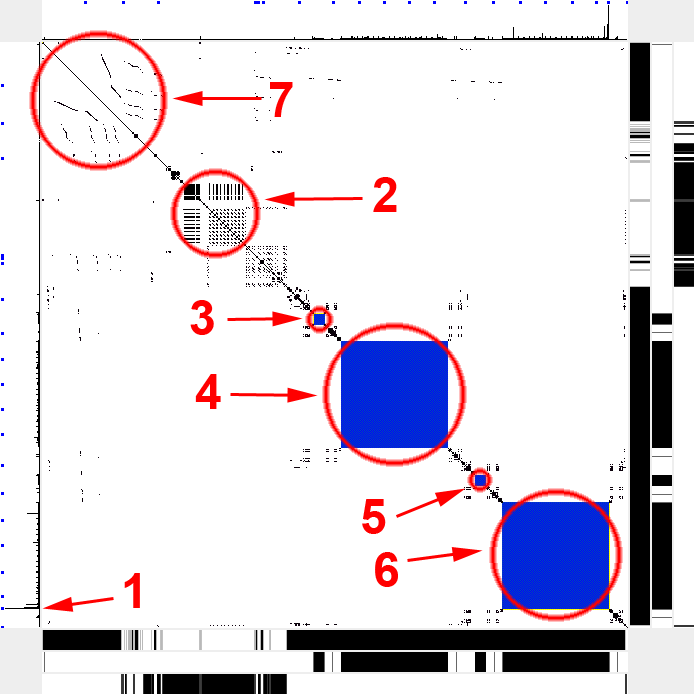
\includegraphics[width=1.0\columnwidth]{dep-cp-xcopy.png}
% \caption{Self-comparison event-ordered \VDP{} of {\tt xcopy}
% copying 8 files of different sizes with the following configuration rules: 
% }
% \begin{tabular}{ll}
% DP match : & operation + parameter (pathname)\\
% DP color : & magenta $\rightarrow$ source; cyan $\rightarrow$ destination;\\
%  & black $\rightarrow$ other\\
% Bar1 color : & black $\rightarrow$ file operation\\
% Bar2 color : & black $\rightarrow$ source/destination files\\
% Bar3 color : & black $\rightarrow$ registry operation
% \end{tabular}
% \label{fig:cp-xcopy}
% \end{center}
% \end{figure}

\begin{figure}[htb]
\begin{center}
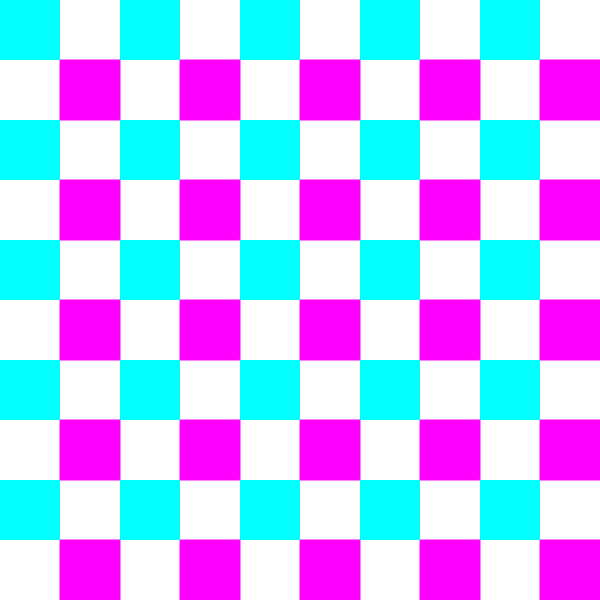
\includegraphics[width=0.10\columnwidth]{dep-cp-zoom.png}
\caption{The alternate zoomed-in view of a blue region in
Fig.~\ref{fig:cp-xcopy} showing reading (magenta) and writing (cyan) operations.
}
\label{fig:cp-zoom}
\end{center}
\end{figure}

We use an example of a simple program and operation,
namely, file copying using \xcopy{}, to explain various
aspects of the \VDP{} visualization.
Fig.~\ref{fig:cp-xcopy} shows a self-comparison event-ordered \VDP{} of
\xcopy{} copying 8 files with sizes
1MB, 10KB, 10MB, 100KB, 1MB, 10KB, 10MB and 100KB and in that given order.
A self-comparison \VDP{} has a 45$^\circ$ diagonal line from top-left to 
bottom-right corner because events on the diagonal always match.
The structure of the files being copied is visible as blue squares in
Region {\em 3}, {\em 4}, {\em 5} and {\em 6} which show copying the
first 1MB and 10MB, then the second 1MB and 10MB files.
It is interesting to see the effect of scale on the visualization.
At this scale, which shows everything, the relative file sizes are also
visible for the large files.  The smaller 10KB and 100KB files are 
too small to be seen at this scale but are visible when zoomed in.
By correlating Bar1 and Bar2,
we find that there are some file related operations in the early phase,
but those files are neither source nor destination files of \xcopy{}.
This might seem surprising. To answer that question, we
click on Region 7, which shows that
the files in question are DLLs. Thus, the top-left region 
shows \xcopy{} loading DLLs.

Bar3 shows that Region {\em 2} has many registry operations which might
be surprising for a file copying task.
% This shows that a command line program can also have many
% registry operations.
The histogram spike at Region 1 shows that some events at the end of the
trace take a long time.
Fig.~\ref{fig:cp-zoom} is a zoomed-in view to one of the blue squares in
Fig.~\ref{fig:cp-xcopy}.
The checkerboard-like pattern shows alternating read (magenta) and write
(cyan) operations which is what we expect for file copy.
Since $cyan+magenta=blue$,
this explains that the blue squares in Fig.~\ref{fig:cp-xcopy} represents
reading from source files and writing to destination files.
We see also that visualizations at different scales can be used for
different purposes.
The extreme magnification in Fig.~\ref{fig:cp-zoom}
shows the actual operations but may be too detailed a view for
the overall picture which emerges at the other extreme in 
Fig.~\ref{fig:cp-xcopy}.

\begin{figure}[tbh]
\begin{center}
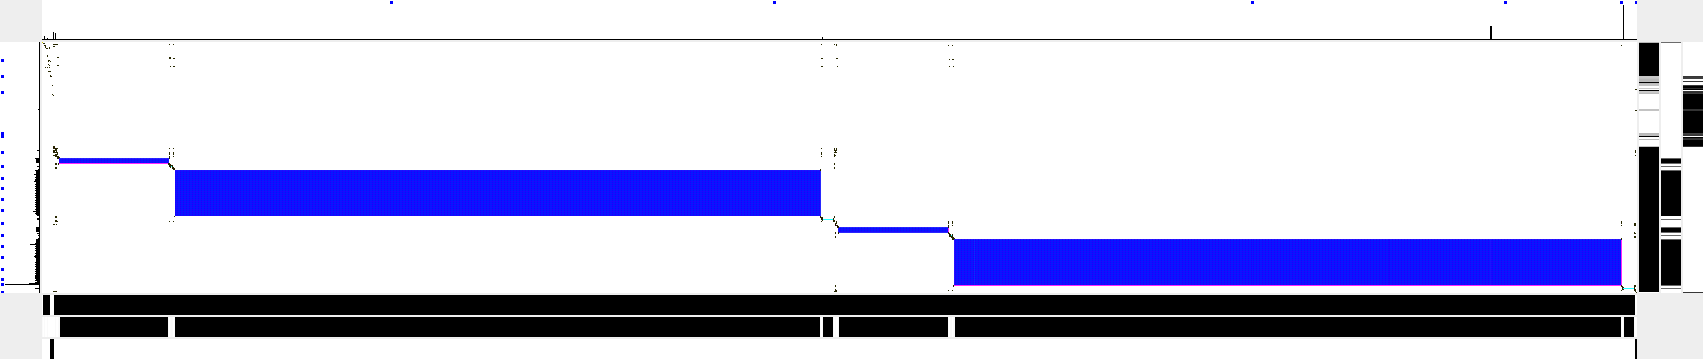
\includegraphics[width=1.0\columnwidth]{dep-cp-xvc.png}
\caption{Event-ordered \VDP{} comparing {\tt cp} (x-axis) and {\tt xcopy} (y-axis) copying
the same files. 
The configurations are the same as in Fig.~\ref{fig:cp-xcopy}.
}
\label{fig:cp-xvc}
\end{center}
\end{figure}
%
\begin{figure}[htb]
\begin{center}
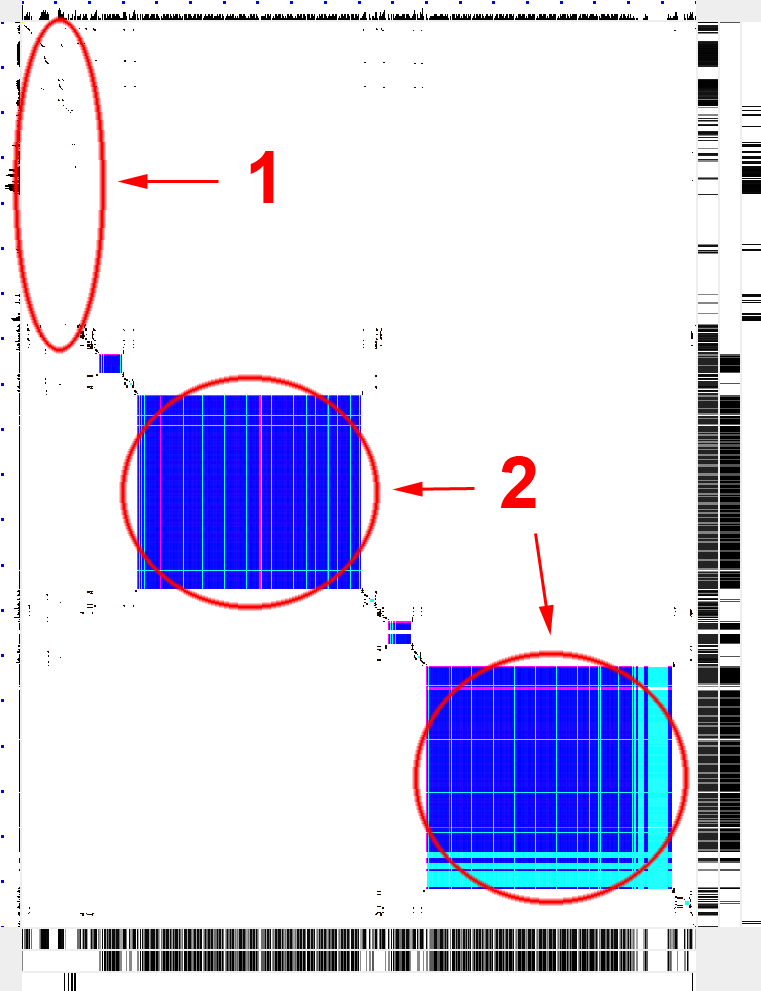
\includegraphics[width=0.6\columnwidth]{dep-cp-64k.png}
\caption{Time-ordered \VDP{} comparing {\tt cp-64k} (x-axis)
and {\tt xcopy} (y-axis).
The configurations are the same as in Fig.~\ref{fig:cp-xcopy}.
}
\label{fig:cp-64k}
\end{center}
\end{figure}

In general, a \VDP{} is used with two traces rather than a single
trace as in a self-\VDP{}.
% Fig. \ref{fig:cp-xcopy} shows a \VDP{} which compares of a {\tt xcopy}
% trace against itself, i.e. a self-similarity comparison.
% Two different traces can also be compared with one trace on the X axis
% and the other trace on the y-axis.
Fig.~\ref{fig:cp-xvc} compares {\tt cp} (x-axis: a Windows version
of GNU {\tt cp}) and {\tt xcopy} (y-axis) copying the same 8 files.
% {\tt cp} is the Windows version of the file copying program included
% in GNU coreutils.
The \VDP{} is much wider than its height, giving
wide blue rectangles instead of blue squares 
(Fig.~\ref{fig:cp-xvc} versus Fig.~\ref{fig:cp-xcopy}).
% \TODO{double check width:height, shouldnt it be 16x?}
% Measuring the width and height of the rectangle,
% we find the ratio of width to height is approximately ? times.
Thus, {\tt cp} performs many more operations than {\tt xcopy}.
To investigate further, zooming in and examining individual events, 
we find that each read and write operation uses a buffer size of 4K,
while {\tt xcopy} uses 64K.
This means that {\tt cp} has 16 times more read and write operations
than {\tt xcopy}.
This is consistent with the width-height ratio in the visualization.

% \begin{figure}[htb]
% \begin{center}
% \includegraphics[width=1.0\columnwidth]{dep-cp-xvct.png}
% \caption{Same as Fig.~\ref{fig:cp-xvc} but the axises are in time units.}
% \label{fig:cp-xvct}
% \end{center}
% \end{figure}

In order to compare the performance of {\tt cp} and {\tt xcopy},
we can use a time-ordered \VDP{}.
% In time based \VDP{}, events are distributed on the axises based on their
% relative time to the first event, while in event based \VDP{}
% events are distributed uniformaly.
Changing the visualization to a time-ordered one (not shown)
shows that {\tt cp} runs slower than {\tt xcopy} though less than 16x.
We then modified {\tt cp} to obtain another version
{\tt cp-64k} which uses 64K buffers.
Fig.~\ref{fig:cp-64k} shows the time-ordered \VDP{} comparing
{\tt cp-64k} (x-axis) and {\tt xcopy} (y-axis).
From Region {\em 2}, we can see that copying of the largest file
is performed in about the same time in both programs.
However, {\tt xcopy} has a slow initialization 
(as shown in Fig.~\ref{fig:cp-64k} Region {\em 1} which includes the registry
operations in Fig.~\ref{fig:cp-xcopy} Region {\em 2}),
which causes {\tt xcopy} to be slower in total than {\tt cp-64k}.

% \TODO{discuss flexible configuration and exploration process also shown
% in the other case studies}


